\documentclass[tikz]{standalone}

\begin{document}
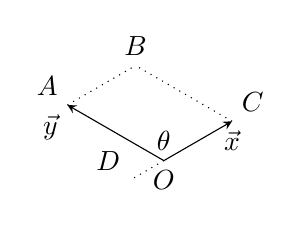
\begin{tikzpicture}
  \draw[->,>=stealth,variable=\r,domain=0:1]
    plot( {\r*cos(30)}, {\r*sin(30)} ) node[below] {\(\vec{x}\)} node[above right] {\(C\)};
  \draw[->,>=stealth,variable=\r,domain=0:1.4142]
    plot( {\r*cos(150)}, {\r*sin(150)} ) node[below left] {\(\vec{y}\)} node[above left] {\(A\)};
  \node[above] at (0,0) {\(\theta\)} node[below] {\(O\)};
  \draw[variable=\r,domain=0:1,dotted]
    plot( {-1.224744872+\r*cos(30)}, {0.7071067810+\r*sin(30)} ) node[above] {\(B\)};
  \draw[variable=\r,domain=0:1.4142,dotted]
    plot( {0.8660254040 + \r*cos(150)}, {0.5+\r*sin(150)} );
  \draw[variable=\r,domain=0:0.5,dotted]
    plot( {\r*cos(210)}, {\r*sin(210)} ) node[above left] {\(D\)};
\end{tikzpicture}
\end{document}
